\chapter{Underground Seismic Noise}

\section{Seismic Noise}
\subsection{Overview}
...\\
...\\
...\\
...\\
...\\
...\\

\subsection{Microseisms}
Microseisms which power spectrum has peaks in $50$--$200\,\mathrm{mHz}$ are excitated by oceanic waves. These seismic waves can be categolized by the generating mechanism of these \cite{Bormann2012new}.

The primary ocean microseisms are generated only in shallow waters in coastal regions. In this regions, the water wave enery can be converted directly into seismic energy either through vertical water pressure variations, or by the impacts of surf on the shores. There are correlation between this microseismic peak and the swell at the beaches was known starting from the data sets studied by \cite{haubrich1963comparative}.
\\
...\\
...\\

The secondary ocean microseisms could be explained by the superposition of ocean waves of equal period traveling in opposite directions. Therefore, generating standing gravity waves of half the period \cite{longuet1950theory}. 
\\
...\\
...\\

The RMS amplitude spectral of both type of the microseisms are strongly depends on the low pressure on the ocean.
\\
...\\
...\\

\begin{figure}[h]
  \begin{center}
    \begin{minipage}[b]{0.65\hsize}
      \centering
      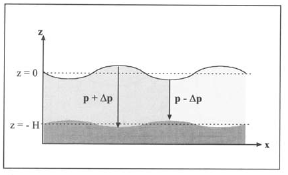
\includegraphics[width=9.0cm]{./img_chap3/img311.png}
      \subcaption{Generating mechanism of the primary microseisms.}\label{img:img311}
    \end{minipage}
    \begin{minipage}[b]{0.65\hsize}
      \centering      
      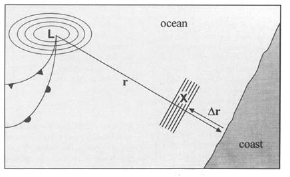
\includegraphics[width=9.0cm]{./img_chap3/img312.png}
      \subcaption{Generating mechanism of the secondary microseisms.}\label{img:img312}
    \end{minipage}
  \end{center}
  \caption{ Generating mechanism of the microsisms. \subref{img:img311} describes the mechanism of the primary microseisms. \subref{img:img312} describes the mechanism of the secondary microseisms.}
\end{figure}


\subsection{Earthquakes}
(Write how earthquakes disturb the large scale interferometer.)

\subsubsection{Mechanism}



遠方での大きな地震は脈動帯域以下の低周波地面振動を励起し、ロックロスの原因になる。
\subsubsection{Early Earthquake Alert}
Seismonをつかって到来時間を予測し、この低周波地面振動のRMSを抑えるための特別なフィルターに切り替えて、ロックロスをへらす工夫を行っている。
しかし、このフィルターは脈動がうるさいときは再びロックロスの問題を抱えてしまう。
\subsection{Earth Tides}

\section{Long-term Study of the seismic environment at KAGRA}
\subsection{Overview}
\subsection{Experimental Arrangement}
Seismic motion ware acquired using seismometer which is installed on the second floor of the X-end named EXV are. The EXV area is placed under 200 $\mathrm{m}$ from surface of the mountain, and moreover, there are no entrance connected to the outside of the mountain in contrast both the Y-end and Corner area. Therefore, It is can be said that this area relatively quiet area in KAGRA site. 

The seismometer is Trillium 120-QA whose three outputs are proportional to the ground velocity of two horizontal and one vertical respectively. As shown in fig. \ref{img:img316}, the seismometer is covered by the black thermal insulator to reduce the thermal fluctuation. 温度のカップリングについてマニュアルchap3.3を参考にして書く\cite{trillium120manual}.

\begin{figure}[H]
  \begin{center}   
    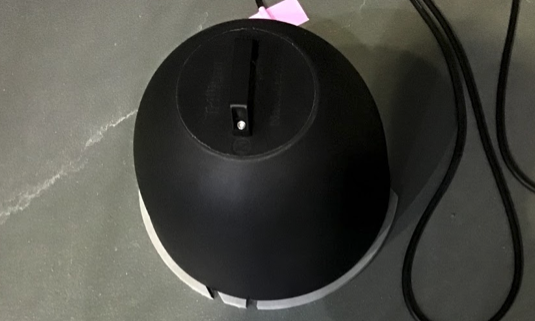
\includegraphics[width=12.0cm]{./img_chap3/img316.png}
    \caption{Trillium 120-QA installed on the second floor at X-end area named EXV area.}\label{img:img316}
  \end{center}
\end{figure}


\subsection{Data Aquisition}



The spectra taken in almost 1 year period using a seismometer at 2nd floor in the X-end station. 


\subsection{Results}
\begin{figure}[H]
  \begin{center}   
    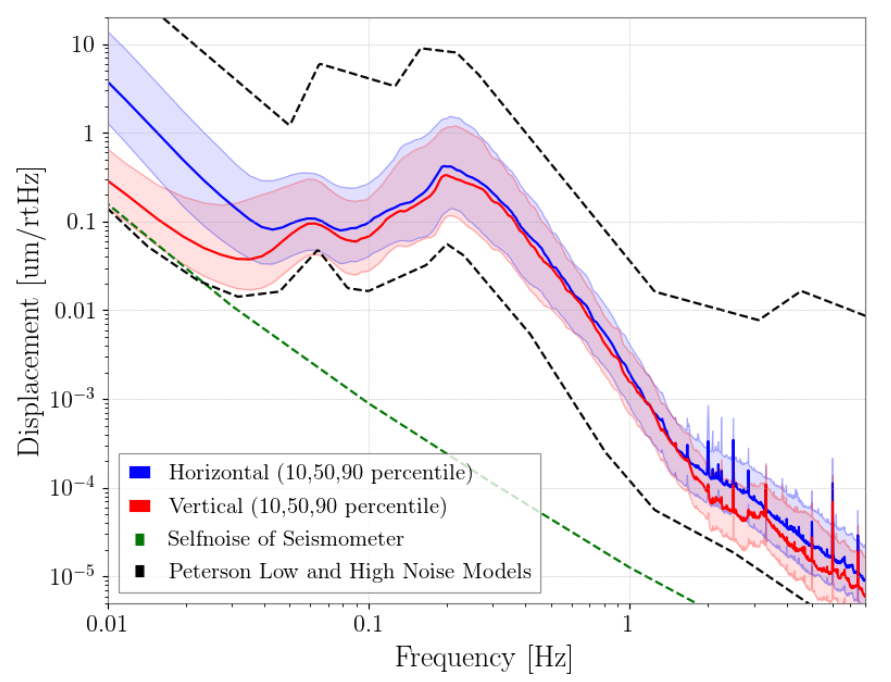
\includegraphics[width=12.0cm]{./img_chap3/img313.png}
    \caption{}
  \end{center}
\end{figure}


huge
\\
...\\
...\\


\subsection{Comparison to Other Site}

\section{Differential Motion Reduction}
\subsection{Introduction}
The motion of two mirrors in the cavity have two modes. One is differential motion, which is the length change of that. Another one is common motion, which is the motion of the center of the cavity. In terms of the length control, it is important that the RMS amplitude of differential motion is as small as possible. Actuarlly, the amplitude of these two motions are the same each other when the mirrors moves with no coherence. However, when a coherence exists, the common motion tends to be larger than the differential one. 

As discussed in this section, the coherence depends on both, the arm length and the wavelength of seismic waves. For example, if the arm length is much more smaller than the wavelength, the mirrors move together. This means that the common motion is greater than the differential motion.

The ratio of the amplitudes of the differential motion over common motion is newly defined as Common and Differential Motion Ratio (CDMR). It is usefull to know how the ground reducts the differential motion or increase the common motion. 

\subsection{Differential Motion Reduction}
\subsubsection{Differential Motion and Common Motion}


\begin{figure}[h]
  \begin{center}
    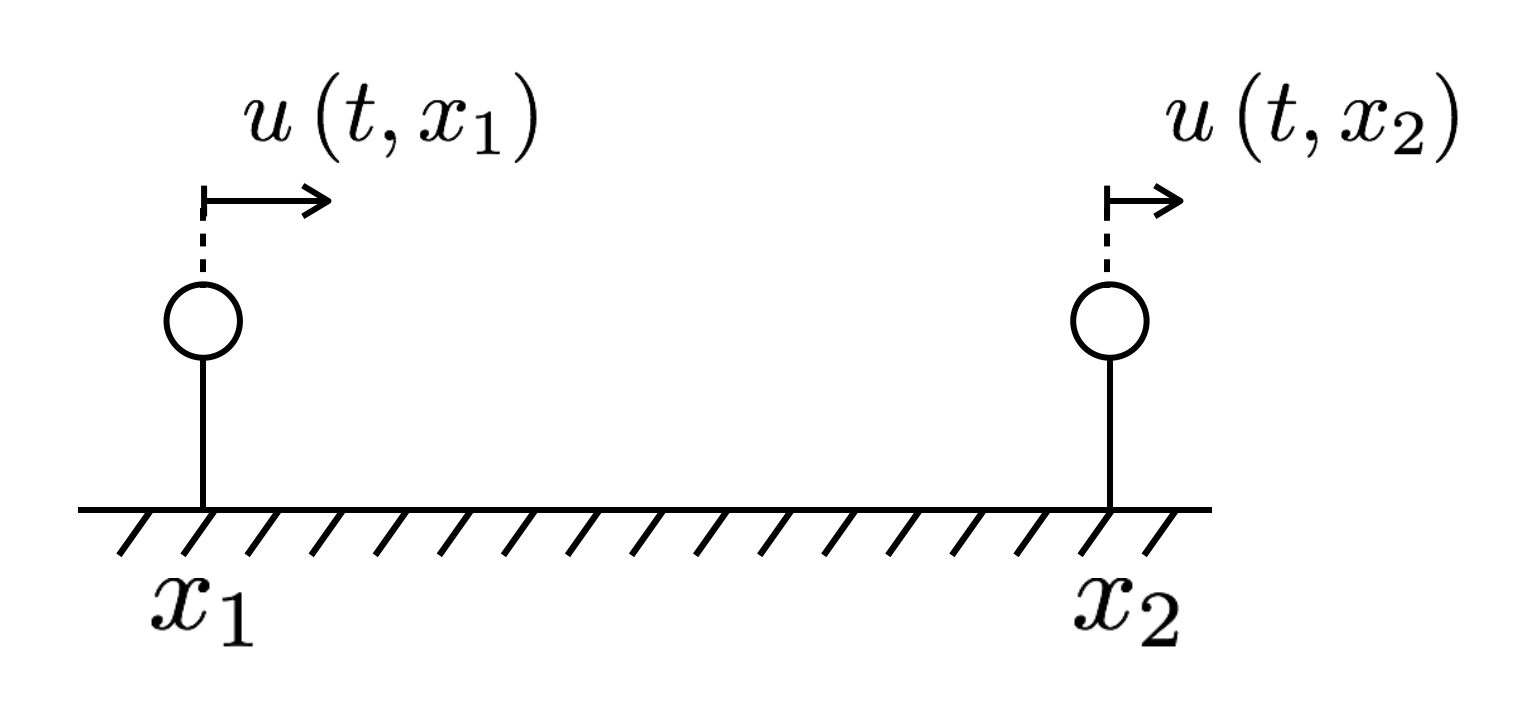
\includegraphics[width=10.0cm]{./img_chap3/img315.png}
    \caption{The displacements of the two points which are sparated L in X axis. }
  \end{center}
\end{figure}


Motions of the two points can be represented as the differential motion and the common motion. Displacement of both differential motion and common motion of the two points shown in Figure(\ref{img:img_chap310}) are defined as
\begin{eqnarray}\label{eq:eq22}
  u_{\mathrm{diff}} \equiv \frac{u_{1}-u_{2}}{\sqrt{2}}, \,
  u_{\mathrm{comm}}  \equiv \frac{u_{1}+u_{2}}{\sqrt{2}}
\end{eqnarray}
where $u_{1}(x,t)$ and $u_2(x,t)$ are the displacement of each points. These two motions defined in Eq.(\ref{eq:eq22}) are normalized by $\sqrt{2}$ due to conserve the total power.


\subsubsection{Common and Differential Motion Ratio (CDMR)}
CDMR is defined as the powers of common motion over the differential motion as bellow,
\begin{equation}
  \mathrm{CDMR} \equiv \sqrt{\frac{\mathrm{Common\,Motion}}{\mathrm{Differential\,Motion}}} = \sqrt{\frac{P_{\mathrm{comm}}(\omega)}{P_{\mathrm{diff}}(\omega)}} \label{eq:eq23}
\end{equation}
where $P_{\mathrm{comm}},P_{\mathrm{diff}}$ are the power spectral densities (PSDs) of the differential motion and common motion, respectively. Each PSDs are converted from the autocorrelation function of these by the Wiener-Khinchin theorem.

First, autocorrelation function $C_{\mathrm{diff}}$ of the differential motion is given by its definition in Eq.(\ref{eq:eq22})
\begin{eqnarray}
  C_{\mathrm{diff}}(\tau) &=& \frac{1}{2}
  \biggl\langle
  \biggl[ x_{1}(t)-x_{2}(t) \biggr] \biggl[ x_{1}(t+\tau)-x_{2}(t+\tau) \biggr]
  \biggr\rangle \\
  &=& \frac{1}{2}\biggl[ C_{11}(\tau) - C_{12}(\tau) - C_{21}(\tau) + C_{22}(\tau) \biggr], 
\end{eqnarray}
,where $C_{ij}$ are the autocorrelation functions of each point and defined as $ C_{ij} \equiv \langle x_{i}(t)x_{j}(t+\tau)\rangle,\, (i=1,2,\,j=1,2)$. Therefore, the power spectrum density of differential motion $P_{\mathrm{diff}}(\omega)$ can be computed as
\begin{eqnarray}
  P_{\mathrm{diff}}(\omega) &=& \frac{1}{2}\biggl[ P_{1}(\omega) + P_{2}(\omega) - P_{12}(\omega) - P_{12}^*(\omega) \biggr]\\
  &=& \frac{1}{2} \biggl[ P_{1}+P_{2} - \mathrm{Re}\left[\gamma \right]\times2\sqrt{P_{1}P_{2}} \biggr] \label{eq:eq31}
\end{eqnarray}
where $P_{1}(\omega),P_{2}(\omega)$ are the power spectrum densities of each points, and $P_{12}(\omega)$ are the cross spectrum between two point. The parameter $\gamma$ is the complex coherence between them defined below,
\begin{eqnarray}
  \gamma \equiv \frac{P_{12}}{\sqrt{P_{1}P_{2}}}.
\end{eqnarray}

Here, assuming that seismic wave propagating each points does not decay, which means $P_{1}=P_{2} \equiv P$, one can compute the $P_{\mathrm{diff}}(\omega)$ as 
\begin{eqnarray}
  P_{\mathrm{diff}}(\omega) = P (1-\mathrm{Re}\left[\gamma\right]).
\end{eqnarray}
Therefore, the PSDs of the common motion can be calculated as
\begin{eqnarray}
  P_{\mathrm{comm}}(\omega) = P (1+\mathrm{Re}\left[\gamma\right]).
\end{eqnarray}
Finaly, CDMR defined Eq.(\ref{eq:eq23}) in case the seismic wave does not decay is represented as
\begin{eqnarray}
 \mathrm{CDMR} = \sqrt{\frac{1 + \mathrm{Re} \left[\gamma \right] }{1 - \mathrm{Re} \left[\gamma \right]}}\,. \label{eq:eq33}
\end{eqnarray}
Eq.(\ref{eq:eq33}) indicate that CDMR can be expressed by only the coherence $\gamma$ between of two points. For example, CDMR tends to be larger when $\gamma$ close to 1. This means that the differential motion is more less than the common motion because the two points move together in the same direction.

\section{Measurement of Differential Motion Reduction}
\subsection{Reduction in X-arm Scale}
\subsection{Reduction in Other Short Scale}



%% \subsubsection{Single Plane Wave Model}
%% The CDMR when single plane wave propagates along the arm cavity is discussed. This model can be applied in the case the source of seismic motion is only one such as an earth quake. Assuming that the plane wave propagates with the azimuth angle $\theta$ along the direction of arm cavity, the wave length $\lambda$ is $\lambda/\mathrm{cos}\theta$. In this situation, the coherence from $x_1$ to $x_2$ is denoted as
%% \begin{equation}
%%   \gamma=e^{i\frac{L\mathrm{cos}\theta\omega}{c}}
%% \end{equation}
%% Therefore, one can compute the CDMR as
%% \begin{equation}  \label{eq:eq18}
%%   \mathrm{CDMR} = \sqrt{\frac{1+\mathrm{cos}(\frac{L\omega}{c}\mathrm{cos}\theta)}{1-\mathrm{cos}(\frac{L\omega}{c}\mathrm{cos}\theta)}}.
%% \end{equation}


%% \subsubsection{Uniform Plane Wave Model}
%% The CDMR when the plane waves are distributed uniformly around the azimuth is discussed. This model can be applied in the case microseisms excite the ground. The coherence is equal to the integral over all direction.
%% \begin{eqnarray} \label{eq:eq19}
%%   \gamma &=& \frac{1}{2\pi} \int_{-\pi}^{\pi} e^{i\frac{\omega}{c} L\cos \theta} d \theta
%% \end{eqnarray}
%% where the coherence is normized azimuth angle. Therefore, the CDMR is given as
%% \begin{equation}  \label{eq:eq20}
%%   \mathrm{CDMR} = \sqrt{\frac{1+J_0(\frac{L\omega}{c})}{1-J_0(\frac{L\omega}{c})}} .
%% \end{equation}





\section{Summary of the Chapter}
